\documentclass[a4paper]{article}

\usepackage{algorithm,amsmath,subfig}
\usepackage[pdftex]{graphicx}
\usepackage[margin=30mm]{geometry}
\usepackage[format=hang,labelfont=it]{caption}
\usepackage[noend]{algorithmic}

\floatname{algorithm}{Listing}
\algsetup{indent=3em}
\renewcommand{\algorithmiccomment}[1]{\quad \{\emph{#1}\}}



\begin{document}
\title{
  \large
  DT8014 Algorithms Group Activities (2014)\\
  \Large
  Week 1 -- Overview and Motivating Examples}
\author{Roland Philippsen}
\maketitle



\noindent
Form groups of 4-5 students and work together on the following tasks.



\section*{Topological Ordering}

\emph{Purpose: a first contact with formalisation, and the difference between verifying -- as opposed to finding -- a solution.}

A \textbf{topological ordering} of a directed graph $G$ is a sequence $L$ of nodes such that, for every edge $(u,v)$, $u$ appears before $v$ in the sequence.
Note that for any path from $u$ to $v$, this also implies that $u$ comes before $v$ in the ordering.
Figure~\ref{fig:topo-order-example} shows an example graph where the sequence of nodes $(C,A,D,B)$ is a topological ordering.

\begin{enumerate}
  
\item
  Suppose you are given a graph $G$ and a sequence of nodes $L$.
  How would you check whether $L$ is a topological ordering of $G$?
  
\item
  The algorithm in Listing~\ref{algo:kahn} computes a topological order.
  Apply it to the graphs in Figures \ref{fig:topo-order-input-a} and \ref{fig:topo-order-input-b}.
  Which one contains a cycle, and where is that cycle?
\end{enumerate}



\section*{Hamiltonian Graphs}

\emph{Purpose: a first contact with combinatorial enumeration.}

A \textbf{Hamiltonian path} is a path in an undirected or directed graph that visits each node exactly once.
A \textbf{Hamiltonian cycle} is a Hamiltonian path that is a cycle, i.e.\ it starts and ends at the same node.
A graph that contains a Hamiltonian cycle is called a \textbf{Hamiltonian graph}.
Figure~\ref{fig:hamiltonian-example} shows an example of such a graph.

\begin{enumerate}
  
\item
  Create two examples of Hamiltonian graphs.
  Then, create two examples of non-Hamiltonian (but connected) graphs.

\item
  For the graph shown in Figure~\ref{fig:hamilton-exercise}, list all the paths that start at node $A$ and visit each node \emph{at most} once (i.e.\ some nodes may remain unvisited).
  Which of these paths are Hamiltonian?
  Which of these paths can be completed into a Hamiltonian cycle?
  
\item
  Suppose you are given a graph $G$ and a sequence of nodes $L$.
  How would you check whether $L$ is a Hamiltonian path in $G$?
  How many steps would your method require -- in the worst case -- for a graph with $N$ nodes?
  
\end{enumerate}



%%%%%%%%%%%%%%%%%%%%%%%%%%%%%%%%%%%%%%%%%%%%%%%%%%


\begin{figure}[H]
  \centering
  \subfloat[]{\label{fig:topo-order-example}
    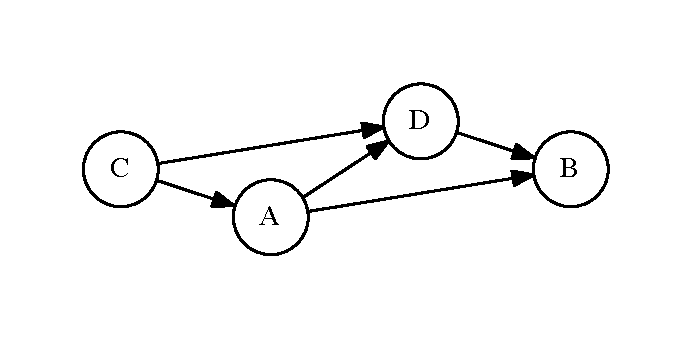
\includegraphics[width=0.4\columnwidth,trim=1cm 1cm 1cm 1cm]{fig/dag-small.pdf}}
  \subfloat[]{\label{fig:topo-order-input-a}
    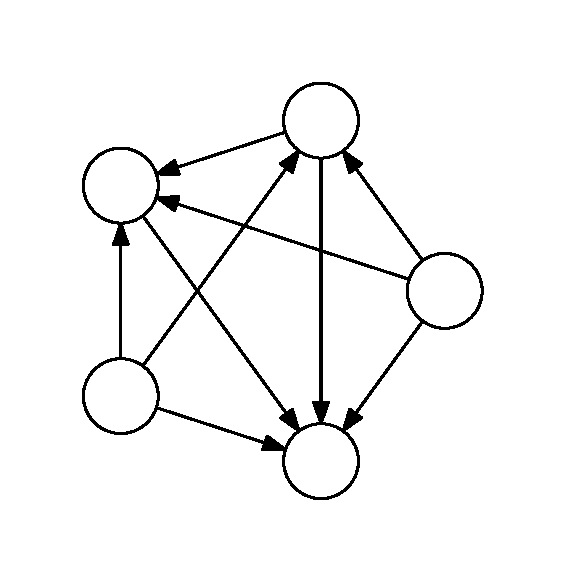
\includegraphics[width=0.28\columnwidth,trim=1cm 1cm 1cm 1cm]{fig/cycle-detection-dag.pdf}}
  \subfloat[]{\label{fig:topo-order-input-b}
    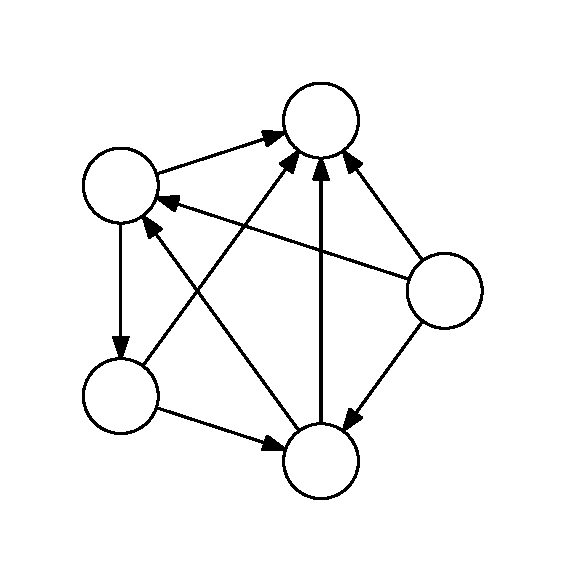
\includegraphics[width=0.28\columnwidth,trim=1cm 1cm 1cm 1cm]{fig/cycle-detection-non-dag.pdf}}
  \caption{
    \textbf{(a)} example DAG arranged from left to right according to topological order.
    \textbf{(b)}~and~\textbf{(c)} example graphs for computing a topological ordering.
  }\label{fig:topo-order}
\end{figure}

\begin{algorithm}
  \caption{
    Kahn's Algorithm\\
    \textbf{Input:} a directed graph $G$
  }\label{algo:kahn}
  \begin{algorithmic}
    \STATE $L \leftarrow$ empty list \COMMENT { will contain the topological order }
    \STATE $S \leftarrow$ set of nodes that have \textbf{no incoming} edges
    \WHILE { $S \neq \emptyset$ }
      \STATE remove a node $n$ from $S$
      \STATE insert $n$ into $L$
      \FORALL [visit all outgoing edges] { edges $e = (n,m)$ }
        \STATE remove $e$ from $G$
        \IF { $m$ has no more incoming edges }
          \STATE insert $m$ into $S$
        \ENDIF
      \ENDFOR
    \ENDWHILE
    \IF { $G$ has edges }
      \RETURN error \COMMENT { $G$ has at least one cycle }
    \ENDIF
    \RETURN $L$
  \end{algorithmic}
\end{algorithm}

\begin{figure}[H]
  \centering
  \subfloat[]{\label{fig:hamiltonian-example}
    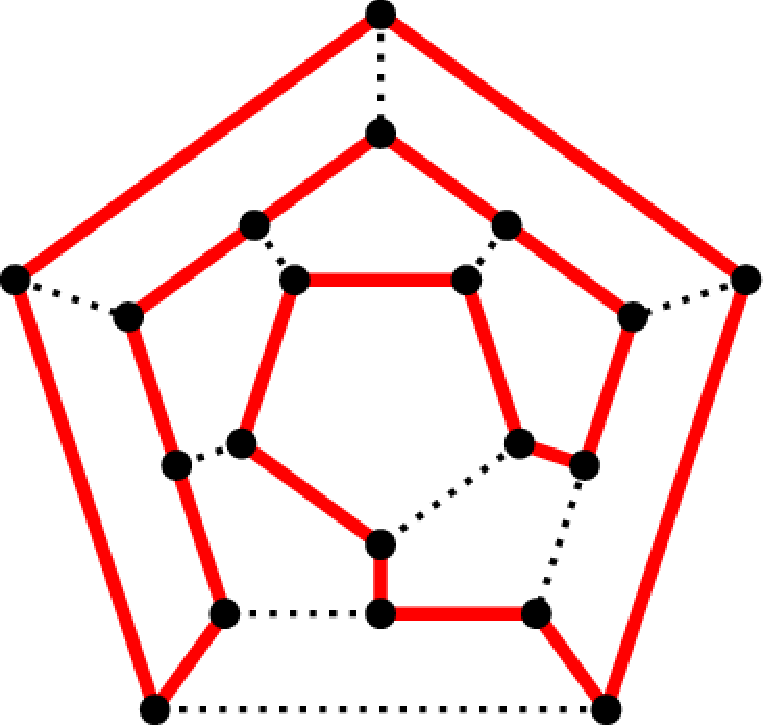
\includegraphics[width=0.25\columnwidth]{fig/hamiltonian-cycle-wikipedia.pdf}}
  \hspace{5mm}
  \subfloat[]{\label{fig:hamilton-exercise}
    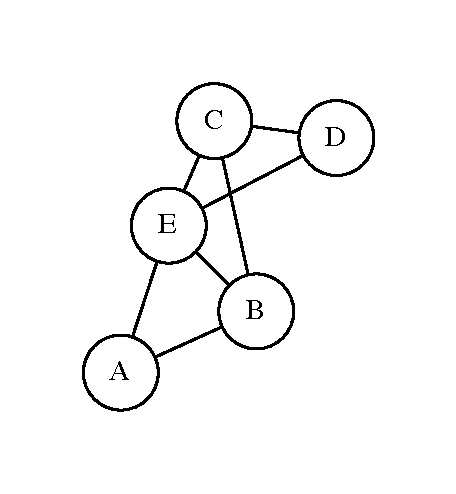
\includegraphics[width=0.3\columnwidth,trim=1cm 1cm 1cm 1cm]{fig/hamilton-exercise.pdf}}
  \caption{
    \textbf{(a)} Hamiltonian cycle taken from \url{http://en.wikipedia.org/wiki/Hamiltonian\_path}.
    \textbf{(b)}~find all Hamiltonian paths starting at $A$ and all Hamiltonian cycles in this graph.
  }
\end{figure}

\end{document}
